% Options for packages loaded elsewhere
\PassOptionsToPackage{unicode}{hyperref}
\PassOptionsToPackage{hyphens}{url}
%
\documentclass[
]{book}
\usepackage{lmodern}
\usepackage{amssymb,amsmath}
\usepackage{ifxetex,ifluatex}
\ifnum 0\ifxetex 1\fi\ifluatex 1\fi=0 % if pdftex
  \usepackage[T1]{fontenc}
  \usepackage[utf8]{inputenc}
  \usepackage{textcomp} % provide euro and other symbols
\else % if luatex or xetex
  \usepackage{unicode-math}
  \defaultfontfeatures{Scale=MatchLowercase}
  \defaultfontfeatures[\rmfamily]{Ligatures=TeX,Scale=1}
\fi
% Use upquote if available, for straight quotes in verbatim environments
\IfFileExists{upquote.sty}{\usepackage{upquote}}{}
\IfFileExists{microtype.sty}{% use microtype if available
  \usepackage[]{microtype}
  \UseMicrotypeSet[protrusion]{basicmath} % disable protrusion for tt fonts
}{}
\makeatletter
\@ifundefined{KOMAClassName}{% if non-KOMA class
  \IfFileExists{parskip.sty}{%
    \usepackage{parskip}
  }{% else
    \setlength{\parindent}{0pt}
    \setlength{\parskip}{6pt plus 2pt minus 1pt}}
}{% if KOMA class
  \KOMAoptions{parskip=half}}
\makeatother
\usepackage{xcolor}
\IfFileExists{xurl.sty}{\usepackage{xurl}}{} % add URL line breaks if available
\IfFileExists{bookmark.sty}{\usepackage{bookmark}}{\usepackage{hyperref}}
\hypersetup{
  pdftitle={Metradica},
  pdfauthor={Marion Boisseaux},
  hidelinks,
  pdfcreator={LaTeX via pandoc}}
\urlstyle{same} % disable monospaced font for URLs
\usepackage{longtable,booktabs}
% Correct order of tables after \paragraph or \subparagraph
\usepackage{etoolbox}
\makeatletter
\patchcmd\longtable{\par}{\if@noskipsec\mbox{}\fi\par}{}{}
\makeatother
% Allow footnotes in longtable head/foot
\IfFileExists{footnotehyper.sty}{\usepackage{footnotehyper}}{\usepackage{footnote}}
\makesavenoteenv{longtable}
\usepackage{graphicx,grffile}
\makeatletter
\def\maxwidth{\ifdim\Gin@nat@width>\linewidth\linewidth\else\Gin@nat@width\fi}
\def\maxheight{\ifdim\Gin@nat@height>\textheight\textheight\else\Gin@nat@height\fi}
\makeatother
% Scale images if necessary, so that they will not overflow the page
% margins by default, and it is still possible to overwrite the defaults
% using explicit options in \includegraphics[width, height, ...]{}
\setkeys{Gin}{width=\maxwidth,height=\maxheight,keepaspectratio}
% Set default figure placement to htbp
\makeatletter
\def\fps@figure{htbp}
\makeatother
\setlength{\emergencystretch}{3em} % prevent overfull lines
\providecommand{\tightlist}{%
  \setlength{\itemsep}{0pt}\setlength{\parskip}{0pt}}
\setcounter{secnumdepth}{5}
\usepackage{booktabs}
\usepackage{booktabs}
\usepackage{longtable}
\usepackage{array}
\usepackage{multirow}
\usepackage{wrapfig}
\usepackage{float}
\usepackage{colortbl}
\usepackage{pdflscape}
\usepackage{tabu}
\usepackage{threeparttable}
\usepackage{threeparttablex}
\usepackage[normalem]{ulem}
\usepackage{makecell}
\usepackage{xcolor}
\usepackage[]{natbib}
\bibliographystyle{plainnat}

\title{Metradica}
\author{Marion Boisseaux}
\date{2022-01-31}

\begin{document}
\maketitle

{
\setcounter{tocdepth}{1}
\tableofcontents
}
\hypertarget{about}{%
\chapter{About}\label{about}}

\emph{to describe}

\hypertarget{part-part-one-general-introduction}{%
\part{Part one: general introduction}\label{part-part-one-general-introduction}}

\hypertarget{background}{%
\chapter{Background}\label{background}}

\begin{itemize}
\tightlist
\item
  Tropical ecosystems, Amazon basin, focus on French Guiana
\item
  Threats : droughts
\item
  Trait-based ecology to define species strategies; a mechanistic understanding with hydraulic traits
\end{itemize}

\hypertarget{project-introduction}{%
\chapter{Project introduction}\label{project-introduction}}

My thesis is 100\% involved in the METRADICA strategic project lead by Clement Stahl and Ghislain Vieilledent. \textbf{Mechanistic traits to predict shifts in tree species abundance and distribution with climate change in the Amazonian forest}.

The global objectives of Metradica are to estimate species vulnerability to climate change and predict shifts in species distribution from species traits.

It combines: current species distribution, hydrological indices, climatic predictions, and use a few key traits at the individual level in innovative models (joint species distribution model; JSDMs), in order to better understand the processes by which species interact with their environment.

There are 4 tasks :

\begin{enumerate}
\def\labelenumi{\arabic{enumi}.}
\tightlist
\item
  environmental index + species hydrological affinity
\item
  species distribution + functional responses to env't\\
\item
  prediction of species distribution from traits using \emph{four-corners} joint species distribution models
\item
  shifts in species distribution through the lens of demographic process: interaction between models
\end{enumerate}

\begin{figure}
\centering
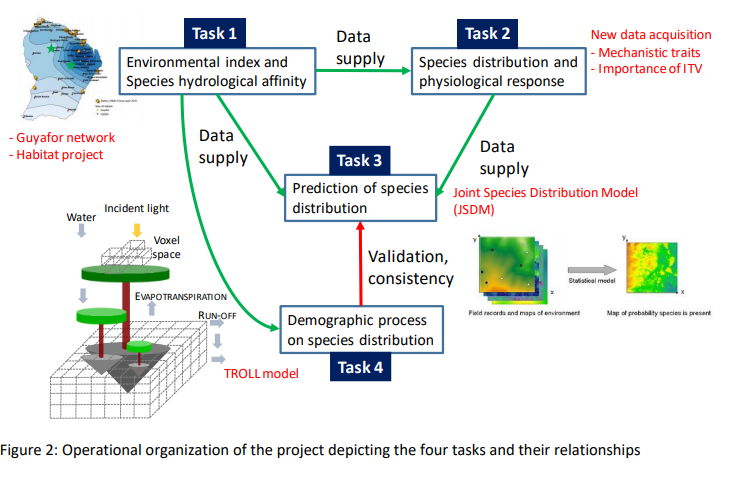
\includegraphics{Metradica_Paracou/Document/Pictures/Overall_project.png}
\caption{METRADICA}
\end{figure}

I am involved in task 2 : to acquire additional traits information in order to have an understanding of the environmental effect on intra- and inter- specific trait variability for morpho-anatomic and mechanistic traits at regional and local scales.

\hypertarget{hypotheses}{%
\chapter{Hypotheses}\label{hypotheses}}

\textbf{(1) Importance of local habitat in shaping functional strategies}

\begin{itemize}
\tightlist
\item
  Habitats are widely recognized to control trait variation
\item
  Identify species with statistically significant habitat associations
\item
  Traits syndromes for specialists vs.~generalists
\end{itemize}

\textbf{(2) Patterns of functional responses to drought along a precipitation and topographic gradient}

\begin{itemize}
\tightlist
\item
  Explore how trait values vary across a precipitation gradient (Bafog ``dry'' to Kaw ``wet'')
\item
  Are associations among traits consistent along the gradient in each habitat? Species should converge to a set of trait values that maximize their resource use efficiency. (Vleminckx et al 2021)
\item
  Identify species in their limit range regarding drought resistance.
  \textbf{(3) Evaluating the inter- and intra-specific variation of hydraulic and leaf traits}
\end{itemize}

Metradica data : exploring generalists species ITV (\textasciitilde60 individuals per species)
Hypothesis : because species' responses to the environment manifest through functional traits, the higher the ITV of a species is, the more diverse abiotic environments the species may be able to adapt to (Umaña et al., 2015).

\hypertarget{part-part-two-materials-method}{%
\part{Part two : Materials \& Method}\label{part-part-two-materials-method}}

\hypertarget{sampling}{%
\chapter{Sampling}\label{sampling}}

\hypertarget{habitats}{%
\section{Habitats}\label{habitats}}

Two main forest habitats are present in French Guiana, \emph{terra firme} (high clay content and high water drainage) and \emph{seasonally flooded forests} (nutrient rich soils and at least 3 months of annual flooding) (INSERER BIBLIO Ferry, 2010). The water table is never observed to descend below 60 cm depth and remains at the soil surface for at least two consecutive months each year (Baraloto et al., 2007; Ferry et al., 2010).
During the field campaigns, we ensure that all trees sampled correspond to the correct habitat. In this case, any errors of habitat classification on the maps are being rectified.

The habitat classification of the tree species are based on all the past project achieved.

\hypertarget{hydrological-indexes}{%
\subsection{Hydrological indexes}\label{hydrological-indexes}}

Topographic variables are strong proxies for soil hydrology, which correlates with a combination of physico-chemical properties. A new hydrological index that accounts for both variations in climate and soil / topography across sites by combining the concept of MCWD with the one of Relative Extractable Water (e.g.~Wagner et al.~2011) or Plant Available Water capacity (Nepstad et al.~2004, Ouédraogo et al.~2016). For Paracou, there is the topography classification established by Allié, Pélissier et al., 2015. \emph{Sylvain}: The topographic wetness index (𝑇𝑊𝐼), identifies water accumulation areas. TWI was derived from 185 a 1-m resolution digital elevation model built based on data from a LiDAR campaign done in 186 2015 using SAGA-GIS (Conrad et al.~2015).

\hypertarget{how-do-we-define-seasonally-flooded-soils}{%
\subsection{How do we define seasonally flooded soils?}\label{how-do-we-define-seasonally-flooded-soils}}

On maps, pixels located at an altitude difference of less than 2 m from the altitude of the nearest surface run-off of the same catchment area. \emph{pixels situés à moins de 2m de dénivelé du plus proche écoulement de surface appartenant au même bassin versant}. Surface run-off corresponds to pixels receiving the waterflow of at least 75 pixels upstream. Everything is being calculated from the SRTM 30 m (after adjusting the basin area with fillings.)

Gaelle information:

\begin{itemize}
\tightlist
\item
  utilisation couche sig onf
\item
  critere pente (inf 20° = BF, pente moins forte espece de lissage avec bc d'arbres en BF, durcissement des criteres, affiner et bien tomber dans du BF) \emph{comment:} SRTM pente 20° à 30m ne correspond pas n'ont plus à la pente sur le terrain, il y a une imprecision. but again in natura we make sure the tree is really in the corresponding habitat.
\item
  distance à la crique (inf 50m) (marginale)
\end{itemize}

The classification in the waterlogged habitat may be loose and not as precise as for the \emph{terra firme}, but it does not impact the sampling. As we mentioned above, \emph{in natura} we assess if the tree is really in a waterlogegd habitat or not.

\hypertarget{sites}{%
\section{Sites}\label{sites}}

Permanent forest plots of the Guyafor network monitor since 1970 (Bafog, Paracou) individual tree growth and mortality in order to understand the different drivers of forest dynamics, including climate and disturbance. The network coves \textgreater{} 235 ha of tropical forest on 12 experimental sites. They are co-managed by the Cirad, CNRS and ONF institutes. METRADICA leaf samplings took place in the control plots.

\begin{figure}
\centering
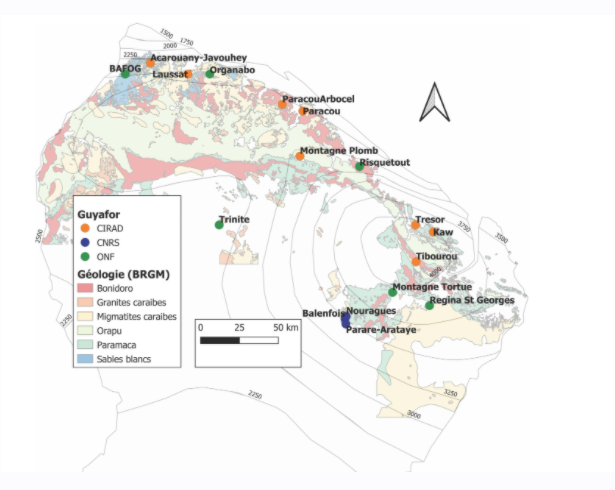
\includegraphics{Metradica_Paracou/Document/Pictures/Guyafor.png}
\caption{Guyafor stations for tropical forest monitoring}
\end{figure}

\textbf{Paracou }: 9 of these permanent forest plots were subjected to 3 different forest exploitation treatments. Out of 9, 3 plots served as control plots. In 1992, 3 additional biodiversity / control plots of 6.25 ha in size and one 25 ha plot were established. Within these plots all trees with a diameter at breast height (DBH) above 10 cm were mapped. Species richness at Paracou ranges between 150 and 200 species per hectare. Since the establishment of the permanent forest plots, tree inventories take place at Paracou, recording tree status (alive or dead) and the DBH to the nearest 0.5 cm. Samplings were done in plots 6, 11, 13, 14, 15, and 16 from the 23/10/2020-7/12/2020 and from 13/09/2021- 17/09/2021. 244 trees sampled but 240 individuals with values. Lost 4 individuals (bota error usually)

\textbf{Bafog}: 5 permanent plots monitored of the ONF institute. Samplings were done in plots 2, 3, 4, and 5 and off plots from the 1st to 16th of March 2021.

\textbf{Est}: Samplings were done in plots KawGuyafor (1 ha) and Trésor from the 4th to 23rd of October 2021. Some trees were also sampled outside the plots.

The three sites were chosen in order to sample species along the rainfall gradient.

\begin{figure}
\centering
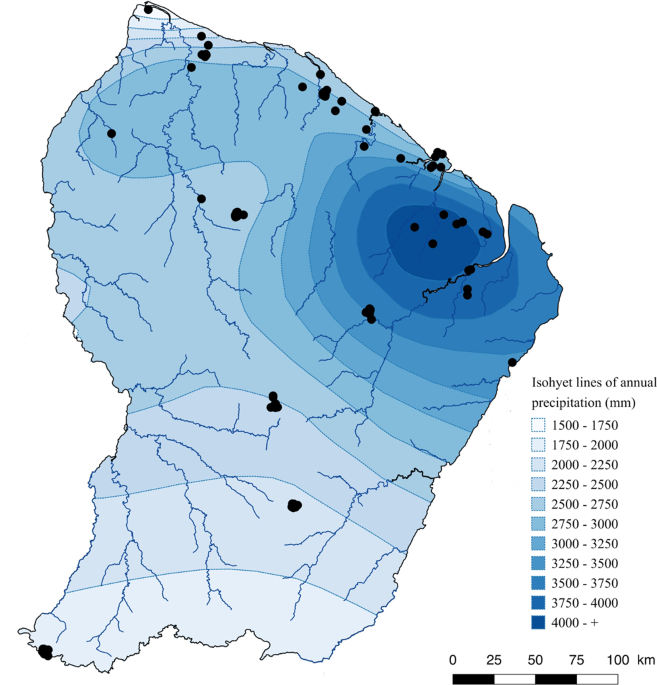
\includegraphics{../Metradica_Paracou/Document/Pictures/41597_2019_218_Fig1_HTML.png}
\caption{Rainfall gradient in French Guyana}
\end{figure}

\hypertarget{species}{%
\section{Species}\label{species}}

\hypertarget{indicator-species-analysis}{%
\subsection{Indicator Species Analysis}\label{indicator-species-analysis}}

We explored the degree of habitat preference using \textbf{Indicator Species Analysis} (Dufrene \& Legendre 1997). It takes account of both relative abundance and relative frequencies of each species across the two main habitats in French Guiana, seasonally flooded forest and Terra firme forests.

\begin{itemize}
\tightlist
\item
  Generalist: IndVal ≠ 0 in the habitats (pVal\textgreater0.08 )
\item
  Specialists: IndVal \textgreater{} 0.24 in one habitat (pVal\textless0.08)
\end{itemize}

Species with high IndVals means that the species prefers the habitat (but not exclusive, hence the word \textbf{preference}), but are also a high probability of being sampled in the given habitat.

Our analysis identified 9 generalist taxa, 8 SFF specialist taxa and 7 terra firme specialist taxa.

\hypertarget{more-details-about-indval}{%
\subsection{More details about IndVal}\label{more-details-about-indval}}

IndVal used by other projects (ex. INSERER BIBLIO TerSteege et al 2013). The relative abundance and the relative frequency must be combined by multiplication because they represent independent information about the species distribution. X100 for a percentage. The index is max when all individuals of a species are found in a single group of sites or when the species occurs in all sites of that group. The statistical significance of the species indicator values is evaluated using a randominization procedure. Significance of habitat association was estimated by a Monte Carlo procedure that reassigns species densities and frequencies to habitats 1000 times. It therefore gives an ecological meaning as it compares the typologies.

Other indicators:

\begin{itemize}
\tightlist
\item
  Contrary to \textbf{TWINSPAN}, this indicator index for a given species is independent of other species relative abundances and there is no need for pseudospecies
\item
  Species richness (sensitive to several factors)
\item
  Oliviera species association to the topographic and edaphic gradient : weighted the HAND or P concentration of the plot by the abundance of the species in the plot. Divided by the number of individuals of the species in all plots.
\end{itemize}

\hypertarget{chosen-species}{%
\subsection{Chosen species}\label{chosen-species}}

Our analysis identified 9 generalist taxa, 8 SFF specialist taxa and 7 terra firme specialist taxa.

\begin{tabular}{l|l|l|l|r|r|r|r|r}
\hline
Family & Genus & Species & Type & Paracou & FTH & ParacouTotal & Bafog & Kaw\\
\hline
Fabaceae & Bocoa & prouacensis & Generalists & 15 & NA & 15 & 10 & 3\\
\hline
Sapotaceae & Chrysophyllum & prieurii & Generalists & 12 & 5 & 17 & 11 & 1\\
\hline
Euphorbiaceae & Conceveiba & guianensis & Generalists & 18 & 2 & 20 & 16 & 0\\
\hline
Lecythidaceae & Eschweilera & coriacea & Generalists & 20 & NA & 20 & 19 & 10\\
\hline
Chrysobalanaceae & Hymenopus & heteromorphus & Generalists & 20 & NA & 20 & 14 & 8\\
\hline
Bignoniaceae & Jacaranda & copaia & Generalists & 18 & 2 & 20 & 12 & 15\\
\hline
Burseraceae & Protium & stevensonii & Generalists & 4 & 8 & 12 & 11 & 1\\
\hline
Fabaceae & Tachigali & melinonii & Generalists & 15 & 1 & 16 & 13 & 13\\
\hline
Myristicaceae & Virola & michelii & Generalists & 6 & 5 & 11 & 16 & 6\\
\hline
Meliaceae & Carapa & surinamensis & SFF specialists & 10 & NA & 10 & 1 & 10\\
\hline
Fabaceae & Eperua & falcata & SFF specialists & 11 & NA & 11 & 0 & 10\\
\hline
Myristicaceae & Iryanthera & hostmannii & SFF specialists & 9 & NA & 9 & 9 & 10\\
\hline
Salicacea & Laetia & procera & SFF specialists & 8 & 1 & 9 & 10 & 10\\
\hline
Burseraceae & Protium & opcaum & SFF specialists & 10 & NA & 10 & 0 & 10\\
\hline
Fabaceae & Pterocarpus & officinalis & SFF specialists & 10 & NA & 10 & 10 & 10\\
\hline
Clusiaceae & Symphonia & globulifera & SFF specialists & 10 & NA & 10 & 9 & 10\\
\hline
Myristicaceae & Virola & surinamensis & SFF specialists & 1 & 5 & 6 & 10 & 10\\
\hline
Salicacea & Casearia & javitensis & TF specialists & 6 & 5 & 11 & 9 & 0\\
\hline
Fabaceae & Dicorynia & guianensis & TF specialists & 6 & NA & 6 & 7 & 0\\
\hline
Lecythidaceae & Gustavia & hexapetala & TF specialists & 4 & 1 & 5 & 9 & 5\\
\hline
Myristicaceae & Iryanthera & sagotiana & TF specialists & 5 & NA & 5 & 5 & 10\\
\hline
Chrysobalanaceae & Licania & membranacea & TF specialists & 5 & NA & 5 & 4 & 5\\
\hline
Metteniusaceae & Poraqueiba & guianensis & TF specialists & 11 & NA & 11 & 10 & 10\\
\hline
Fabaceae & Vouacapoua & americana & TF specialists & 5 & NA & 5 & 7 & 10\\
\hline
\end{tabular}

Un espèce : bc mortlité chez les jeunes donc parti pris de les considerer dans le choix des habitats. (percentile 10-90).
For \emph{Eperua falcata}: BF?? see Laurens porter 2007 (are species adapted \ldots)

\hypertarget{phylogeny}{%
\subsection{Phylogeny}\label{phylogeny}}

We also wanted to maximize the phylogeny to get a greater picture, having specialists and generalists in the main clades: (Rosids, Asterids, Magnoliids). This would allow us to assess whether the different strategies to drought tolerance can be extend to the species of the same clade.

\begin{figure}
\centering

\includegraphics{_main_files/figure-latex/unnamed-chunk-3-1.pdf}
\caption{\label{fig:unnamed-chunk-3}phylogeny}
\end{figure}

\hypertarget{individuals}{%
\section{Individuals}\label{individuals}}

The individuals were selected with a DBH value between the 10th and the 90th percentile of the species' distribution pattern, in order to have a sampling that best reflects the forest structure. In this percentile interval, species were randomly selected for sampling.

Sampling strategy :

\begin{itemize}
\tightlist
\item
  Maps were produced by QGIS software
\item
  \href{../Metradica_Paracou/Document/Protocol/Field.Rmd}{\textbf{Field} protocol}
\item
  Fill the fieldworksheet \href{../Metradica_Paracou/Document/Protocol/Feuille_terrain_releve.xlsx}{\textbf{Fieldworksheet}}
\item[$\square$]
  Assess tree and branch height
\item[$\square$]
  Assess tree and branch Dawkins : 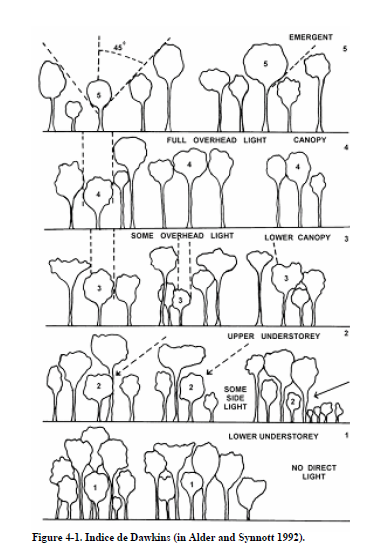
\includegraphics{../Metradica_Paracou/Document/Protocol/Dawkins.png}
\end{itemize}

\hypertarget{summary}{%
\section{Summary}\label{summary}}

\begin{itemize}
\tightlist
\item
  2 habitats (Terra firme; Seasonally flooded soils)
\item
  24 species (9 generalists; 8 SFF; 7 TF)
\item
  10 individuals per species per site
\item
  9 traits to investigate for drought tolerance
\end{itemize}


\includegraphics{_main_files/figure-latex/unnamed-chunk-4-1.pdf}

\begin{table}

\caption{\label{tab:unnamed-chunk-4}Individuals per species collected on the 3 sites}
\centering
\begin{tabular}[t]{l|l|l|l|r|r|r|r|r}
\hline
Family & Genus & Species & Type & Paracou & FTH & ParacouTotal & Bafog & Kaw\\
\hline
Fabaceae & Bocoa & prouacensis & Generalists & 15 & NA & 15 & 10 & 3\\
\hline
Sapotaceae & Chrysophyllum & prieurii & Generalists & 12 & 5 & 17 & 11 & 1\\
\hline
Euphorbiaceae & Conceveiba & guianensis & Generalists & 18 & 2 & 20 & 16 & 0\\
\hline
Lecythidaceae & Eschweilera & coriacea & Generalists & 20 & NA & 20 & 19 & 10\\
\hline
Chrysobalanaceae & Hymenopus & heteromorphus & Generalists & 20 & NA & 20 & 14 & 8\\
\hline
Bignoniaceae & Jacaranda & copaia & Generalists & 18 & 2 & 20 & 12 & 15\\
\hline
Burseraceae & Protium & stevensonii & Generalists & 4 & 8 & 12 & 11 & 1\\
\hline
Fabaceae & Tachigali & melinonii & Generalists & 15 & 1 & 16 & 13 & 13\\
\hline
Myristicaceae & Virola & michelii & Generalists & 6 & 5 & 11 & 16 & 6\\
\hline
Meliaceae & Carapa & surinamensis & SFF specialists & 10 & NA & 10 & 1 & 10\\
\hline
Fabaceae & Eperua & falcata & SFF specialists & 11 & NA & 11 & 0 & 10\\
\hline
Myristicaceae & Iryanthera & hostmannii & SFF specialists & 9 & NA & 9 & 9 & 10\\
\hline
Salicacea & Laetia & procera & SFF specialists & 8 & 1 & 9 & 10 & 10\\
\hline
Burseraceae & Protium & opcaum & SFF specialists & 10 & NA & 10 & 0 & 10\\
\hline
Fabaceae & Pterocarpus & officinalis & SFF specialists & 10 & NA & 10 & 10 & 10\\
\hline
Clusiaceae & Symphonia & globulifera & SFF specialists & 10 & NA & 10 & 9 & 10\\
\hline
Myristicaceae & Virola & surinamensis & SFF specialists & 1 & 5 & 6 & 10 & 10\\
\hline
Salicacea & Casearia & javitensis & TF specialists & 6 & 5 & 11 & 9 & 0\\
\hline
Fabaceae & Dicorynia & guianensis & TF specialists & 6 & NA & 6 & 7 & 0\\
\hline
Lecythidaceae & Gustavia & hexapetala & TF specialists & 4 & 1 & 5 & 9 & 5\\
\hline
Myristicaceae & Iryanthera & sagotiana & TF specialists & 5 & NA & 5 & 5 & 10\\
\hline
Chrysobalanaceae & Licania & membranacea & TF specialists & 5 & NA & 5 & 4 & 5\\
\hline
Metteniusaceae & Poraqueiba & guianensis & TF specialists & 11 & NA & 11 & 10 & 10\\
\hline
Fabaceae & Vouacapoua & americana & TF specialists & 5 & NA & 5 & 7 & 10\\
\hline
\end{tabular}
\end{table}

\hypertarget{traits}{%
\chapter{Traits}\label{traits}}

This chapter defines measured and sampled traits with associated protocols.

\hypertarget{morphological-traits}{%
\section{Morphological traits}\label{morphological-traits}}

\begin{itemize}
\tightlist
\item
  \textbf{LA}: leaf area \(cm^{2}\) : carbo- acquisition related trait which informs on the light capture strategy.
\item
  \textbf{LDMC}: leaf dry matter content \(mg.g^{-1}\) : a carbon-acquisition related trait which informs on the carbon investment in physical resistance and defense.
\end{itemize}

\hypertarget{hydraulic-traits}{%
\section{Hydraulic traits}\label{hydraulic-traits}}

\begin{itemize}
\tightlist
\item
  \textbf{RWC}: relative water content (\%) is of special interest as it reflects the amount of water present the leaf relative to the maximum it can hold (\emph{INSERER BIBLIO Barrs \& Weatherley 1962})
\item
  \textbf{\(\pi_{TLP}\)}: leaf water potential at which leaf cells lose turgor (MPa), a key drought tolerance trait.
\item
  \textbf{\(g_{min}\)}: leaf minimum conductance \(mmol.m^{-2}.s^{-1}\) taking into account water losses through the cuticle and incompletely closed stomata.
\item
  \textbf{Stomatal characteristics (size, density)}: morphological characteristic at the crossroads between water loss and the maximum rate of photosynthesis.(\emph{INSERER BIBLIO Julio V. Schneider 2016})
\item
  \textbf{Nervation density}: determining the capacity of water supply in leaves. (\emph{INSERER BIBLIO Julio V. Schneider 2016})
\item
  \textbf{Leaf chemistry} : To assess the leaves' concentration in carbon, nitrogen and phosphorous.
\item
  \textbf{Pmidday}: Water potential at the driest point of the day.
\item
  \textbf{\(\delta\) 18 O and \(\delta\) 13 C} : Informs patterns of carbon and water use, related to water use efficiency. (\emph{INSERER BIBLIO Farquhar et al 1989}) Measured in Vienna.
\end{itemize}

\hypertarget{photochemical-trait}{%
\section{Photochemical trait}\label{photochemical-trait}}

\begin{itemize}
\tightlist
\item
  \textbf{\(\frac{Fv}{Fm}\)}: maximum quantum yield of photosystem II, which reflects photosynthesis efficiency (\(\mu mol . m^{-2} . s^{-1}/ \mu mol . m^{-2} . s^{-1}\)). It is an indicator of photosynthetic performance, as it has been shown to be sensitive to drought constraints in tropical forests (\emph{INSERER BIBLIO Manzi et al 2021}) but decline after other leaf hydraulic traits (\emph{INSERER BIBLIO Trueba et al 2019}).
\end{itemize}

\hypertarget{measured-traits}{%
\section{Measured traits}\label{measured-traits}}

\begin{itemize}
\tightlist
\item
  Day 1

  \begin{itemize}
  \tightlist
  \item
    Fresh

    \begin{itemize}
    \tightlist
    \item
      On field: Pmidday
    \item
      scan gmin leaves
    \item
      fresh weight RWC
    \item
      \textbf{\(g_{min}\)} weight\\
    \item
      \textbf{Stomatal density} nail polish (3 replicates per indivual)
    \item
      \textbf{\(\frac{Fv}{Fm}\)}
    \end{itemize}
  \item
    Day 2

    \begin{itemize}
    \tightlist
    \item
      saturated weight RWC
    \item
      \textbf{\(g_{min}\)} finish weights (at least 2 points next day)
    \item
      \textbf{\(\pi_{TLP}\)}
    \end{itemize}
  \item
    Day 5 (+72h)

    \begin{itemize}
    \tightlist
    \item
      Dry weight RWC
    \end{itemize}
  \end{itemize}
\item
  Later on :

  \begin{itemize}
  \tightlist
  \item
    Stomatal observation and density counts
  \item
    Measure of vein densities
  \item
    Chemistry of dry-grinded leaves
  \end{itemize}
\end{itemize}

\hypertarget{protocols}{%
\section{Protocols}\label{protocols}}

\begin{itemize}
\tightlist
\item
  \href{../Metradica_Paracou/Document/Protocol/Field.Rmd}{\textbf{Field} protocol}
\item
  \href{../Metradica_Paracou/Document/Protocol/Protocole_Ptlp.pdf}{\textbf{\(\pi_{TLP}\)} protocol}
\item
  \href{../Metradica_Paracou/Document/Protocol/RWC_Boisseaux.docx}{\textbf{RWC} protocol}
\item
  \href{../Metradica_Paracou/Document/Protocol/Analyse\%20Stomates_Marion.docx}{\textbf{Stomata} protocol}
\item
  \href{../Metradica_Paracou/Document/Protocol/Fluo_Bellifa.docx}{\textbf{FvFm} protocol}
\item
  \href{../Metradica_Paracou/Document/Protocol/Gmin\%20protocol.docx}{\textbf{gmin} protocol}
\item
  \href{../Metradica_Paracou/Document/Protocol/ProtocolLeafVeins_MB_2.docx}{\textbf{leaf venation} protocol}
\end{itemize}

\hypertarget{part-part-three-results}{%
\part{Part three : Results}\label{part-part-three-results}}

\hypertarget{pca-results}{%
\chapter{PCA results}\label{pca-results}}

The aim is to define a set of key traits that together explain why a species would be specialist or generalist.

Generalist species should display a greater degree of intraspecific variability in traits related to habitat use than specialists because they experience a wider range of environmental conditions and/or have inherently higher levels of phenotypic plasticity.

Here is an analysis aimed to explore co-variations of individual traits. Specifically, I investigated individual traits co-variation at two taxonomic scales: among species, and within species.

\hypertarget{trait-covariation}{%
\chapter{Trait covariation}\label{trait-covariation}}

\begin{itemize}
\tightlist
\item
  Clean dataset
\end{itemize}

\begin{verbatim}
##   Code idTree Plot Subplot FieldNr pref.Habitat Habitat  spName Fresh_Weight.g.
## 1    1 145493   15       1     182           BF      BF Iry.hos           1.268
## 2    2 147663   15       3     178           TF      TF Gus.hex           1.293
## 3    3 147783   15       3     298           BF      BF Iry.hos           0.877
## 4    4 147625   15       3     140   Generalist      TF Tac.mel           0.258
## 5    5 148586   15       3    1103   Generalist      TF Chr.pri           1.087
## 6    6 149072   15       4     369   Generalist      TF Con.gui           2.196
##   Saturated_Weight.g. Delta_Weight_SW.FW.g. delta_en_._real delta_en_._clean
## 1               1.263                -0.005          -0.379           -0.379
## 2               1.320                 0.027           2.057            2.057
## 3               0.874                -0.003          -0.399           -0.399
## 4               0.256                -0.002          -0.814           -0.814
## 5               1.123                 0.036           3.340            3.340
## 6               2.211                 0.015           0.688            0.688
##   Dry_Weight.g.     RWC  LSWC P_osmo  P_tlp mean_Pmidday Fv.Fm LA..cm.2.
## 1         0.501 100.629 1.523 -1.130 -1.568           NA 0.786    45.231
## 2         0.464  96.890 1.842 -1.560 -1.911           NA 0.797    48.827
## 3         0.349 100.667 1.503 -1.028 -1.486           NA 0.807    41.215
## 4         0.121 101.554 1.118 -1.510 -1.871           NA 0.840     9.776
## 5         0.535  93.831 1.100 -2.403 -2.585       26.067 0.773    31.427
## 6         1.010  98.742 1.188 -1.328 -1.726       21.580 0.800    64.251
##   gmin..mmol.m.2.s.1. X1st_Order_Vein_Density..mm.mm.2.
## 1               1.235                             0.018
## 2               0.916                             0.031
## 3               1.046                             0.031
## 4               3.368                             0.058
## 5               1.869                                NA
## 6               6.776                             0.023
##   X2nd_Order_Vein_Density..mm.mm.2. X3rd_Order_Vein_Density..mm.mm.2.
## 1                             0.241                             0.682
## 2                             0.150                             0.347
## 3                             0.196                             0.640
## 4                             0.277                             0.789
## 5                                NA                                NA
## 6                             0.081                             0.301
##   Major_Vein_Density..mm.mm.2. Stomata_Density..nb.mm.2. Stomata_Size..um.2.
## 1                        0.941                        NA                  NA
## 2                        0.527                        NA                  NA
## 3                        0.867                        NA                  NA
## 4                        1.124                        NA                  NA
## 5                           NA                        NA                  NA
## 6                        0.405                        NA                  NA
##   Height_Tree Dawkin_Tree Height_Branch Dawkin_Branch Position_Crown
## 1          12           4            10             4            Sup
## 2          11           2             9             2            Sup
## 3          12           2            13             3            Sup
## 4          33           5            23             4            Mid
## 5          24           4            21             4            Sup
## 6          15           2            14             3            Sup
\end{verbatim}

We aimed to explore co-variations of leaf traits belonging to 244 individuals from 24 species. We investigated trait co-variation at 2 taxonomic scales: (i) between species, (ii) within species between individuals.

Between all species, \textbf{26.34\%} of the total variance was conserved on the two first axes from the PCA of the traits. The \emph{first axis opposed SLA to CC and LT, from high SLA leaves to thick leaves rich in chlorophyll, whereas the second axis is related to LA and LDMC, increasing with leaf area and dry matter. The first axis highlighted a correlation between CC and LT. SLA and LA decoupled relation is enlightened within the PCA plane. Moreover for the two complexes, we observed a general trend of diameters distribution along the first PCA axis. Smaller diameter seemed linked to thinner leaves with increased SLA and less chlorophyll. Besides both axes showed significative complex segregation (\(p-value < 0.0001\)), the second PCA axis segregated the two complexes with no overlap.}
Les 2 premiers axes de l' analyse expriment \textbf{26.34\%} de l'inertie totale du jeu de données ; cela signifie que 26.34\% de la variabilité totale du nuage des individus (ou des variables) est représentée dans ce plan.
C'est un pourcentage relativement faible, et le premier plan ne représente donc seulement qu'une part de la variabilité contenue dans l'ensemble du jeu de données actif.
Cette valeur est supérieure à la valeur référence de \textbf{14.1\%}, la variabilité expliquée par ce plan est donc significative
(cette intertie de référence est le quantile 0.95-quantile de la distribution des pourcentages d'inertie obtenue en simulant 2209 jeux de données aléatoires de dimensions comparables sur la base d'une distribution normale).

Du fait de ces observations, il serait alors très probablement nécessaire de considérer également les dimensions supérieures ou égales à la troisième dans l'analyse.

\hypertarget{part-part-four-notes}{%
\part{Part four : Notes}\label{part-part-four-notes}}

\hypertarget{section}{%
\chapter{26/01/2022}\label{section}}

Metradica meeting

Presents:

\begin{itemize}
\tightlist
\item
  Ghislain
\item
  Clément\\
\item
  Sabrina
\item
  Damien\\
\item
  Jeanne
\item
  Marion
\end{itemize}

Objectives:

1- les données 13C\\
2- les modèles joints

\textbf{Notes:}

\begin{enumerate}
\def\labelenumi{(\arabic{enumi})}
\item
\end{enumerate}

L'estimation de l'efficience d'utilisation de l'eau intrinsèque peut être obtenue à l'aide de msures directes des échanges gazeux entre feuille et atm. Farquar 1982 propose un modèle simple reliant WUE (water use efficiency) à la discrimination isotopique du C au cours de la photosynthèse.

Relation WUE et \(\delta\) 13C positive.

Drivers de la compo iso:

\begin{itemize}
\tightlist
\item
  Lumière (feuille d'ombre valeurs 13C nettement plus négatives)
\item
  génétique
\item
  sécheresse atm + sol
\item
  VPD
\item
  teneur en mx du sol
\item
  ontogénie de l'individu
\item
  conductance hydraulique
\end{itemize}

Attention: la compo iso n'est pas un trait lié à la sécheresse. Il caractérise \emph{l'acclimation} à la sécheresse. Il est utile pour une expé en serre de comparer le \(\delta\) 13C entre le groupe controle et le groupe dry. Une espèce sensible: on trouvera une forte différence vs.~une espèce peu sensible, une faible différence. Et le \emph{delta} ser aun trait de réponse à la sécheresse.

Travaux de Damien:

\begin{itemize}
\tightlist
\item
  16 parcelles à travers la Guyane
\item
  9-10 sites\\
\item
  \textasciitilde100 arbres / parcelles
\item
  \textasciitilde1600 valeurs de compo iso de feuille d'arbres dominant
\item
  70 espèces différentes avec qq indet. par site; total de 392 espèces identifiées
\item
  Moyenne valeur \(\delta\) 13C \textasciitilde{} -30 \%0 pour les forêts en Guyane
\item
  Lorsque le climat est le même, on observe le même fonctionnement
\end{itemize}

\begin{enumerate}
\def\labelenumi{(\arabic{enumi})}
\setcounter{enumi}{1}
\item
\end{enumerate}

Avant nous procédions par espèces, le but des modèles joints: faire avec plusieurs espèces en même temps.Les modèles joints de distribution des espèces permettent d'estimer la niche des espèces, de prédire leur distribution, tout en prenant en compte les intéractions entre espèces. Ils peuvent être utilisés pour déterminer les communautés ou assemblages d'espèces et comment ces assemblages changent spatialement, selon des gradients environnementaux.

Prendre en compte: la co-occurence des espèces + relation trait-env't pour déterminer la présence d'une espèce sur 1 site.

\begin{figure}
\centering
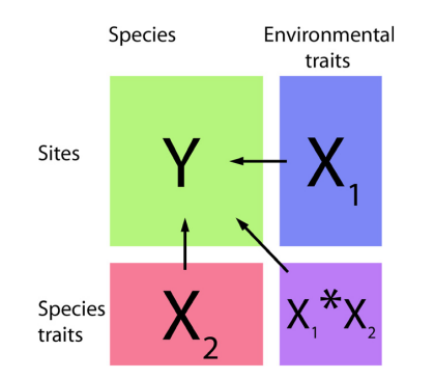
\includegraphics{Metradica_Paracou/Document/Pictures/ModeleJoint.png}
\caption{Modèle joint}
\end{figure}

Si l'on inclu les données 13C dans les modèles joints: on s'attend à une abscence de réponse.

  \bibliography{book.bib,packages.bib}

\end{document}
